% SETUP
\documentclass[11pt]{article}
\linespread{1.15}
\usepackage[english]{babel}
\usepackage[utf8]{inputenc}
\usepackage{graphicx, amsmath, array, graphics, amssymb, epsfig, psfrag, geometry, alltt, subfiles, blindtext, enumitem,float,pdfpages,multicol,tabularx}
\usepackage[export]{adjustbox}
\usepackage{fancyhdr}
\usepackage{array}
\usepackage{hyperref}
%%%%%%%%%%%%%%  code listing
\usepackage{listings}
\usepackage{color} %red, green, blue, yellow, cyan, magenta, black, white
\definecolor{mygreen}{RGB}{2,94,33} % color values Red, Green, Blue
\definecolor{mylilas}{RGB}{170,55,241}
\usepackage{hyperref}
\hypersetup{
    colorlinks=true,
    linkcolor=black,
    filecolor=magenta,      
    urlcolor=blue,
}
\urlstyle{same}
%Includes "References" in the table of contents
\usepackage[nottoc]{tocbibind}

% MATLAB code insert
\lstset{language=Matlab,%
    %basicstyle=\color{red},
    breaklines=true,%
    morekeywords={matlab2tikz},
    keywordstyle=\color{blue},%
    morekeywords=[2]{1}, keywordstyle=[2]{\color{black}},
    identifierstyle=\color{black},%
    stringstyle=\color{mylilas},
    commentstyle=\color{mygreen},%
    showstringspaces=false,%without this there will be a symbol in the places where there is a space
    numbers=left,%
    numberstyle={\tiny \color{black}},% size of the numbers
    numbersep=9pt, % this defines how far the numbers are from the text
    emph=[1]{for,end,break},emphstyle=[1]\color{black}, %some words to emphasise
    %emph=[2]{word1,word2}, emphstyle=[2]{style},    
}
%%%%%%%%%%%%%%%%


\geometry{a4paper, top = 20mm, bottom = 20mm, left = 15mm, right = 15mm}

% Do we need a cover page?

% Headers
\pagestyle{fancy}
\fancyhf{}
\chead{ELEN90066 Embedded System Design - Final Report}
\cfoot{\thepage}

\begin{document}
\includepdf{EngCSAss1.pdf}
\clearpage
\begin{titlepage}

\newcommand{\HRule}{\rule{\linewidth}{0.5mm}}

\begin{center}
% Upper part of the page
\includegraphics[width=\textwidth]{Images/MSE.jpg}\\[1cm]  
\textsc{\Large ELEN90066 - Embedded System Design}\\[0.5cm]
% Title
\HRule \\[0.4cm]
{\bfseries Kobuki Obstacle Course Project}\\[0.4cm]

\large{Final Report}
\HRule \\[2cm]

% Author and supervisor

\begin{minipage}{0.45\textwidth}
\begin{flushleft} \large
\emph{\textbf{Lecturer:}}\\[0.2cm]
\emph{\textbf{Demonstrator:}}\\[0.2cm]
\emph{\textbf{Workshop:}}\\[0.2cm]
\emph{\textbf{Due Date:}}\\[0.2cm]
\emph{\textbf{Students:}}\\[0.2cm]
\vspace{1.3cm}
\end{flushleft}
\end{minipage}
\begin{minipage}{0.45\textwidth}
\begin{flushright} \large
Gavin Buskes \\[0.2cm]
Bigi Philips \\[0.2cm]
Monday 15:15pm - 18:15pm (Group 9)\\[0.2cm]
04/11/19\\[0.2cm]
Craig Reid [756879]\\[0.2cm] 
Xiuwen Peng [825801]\\[0.2cm]
YiLin Inez Zheng [702279]
\end{flushright}
\end{minipage}
\vfill
% Bottom of the page
{\large \today}
\end{center}
\end{titlepage}

% Title
\begin{center}
\textbf{\Large{Kobuki Obstacle Course Project - Final Report}}
\end{center}

\vspace{-0.5cm}
\section*{Executive Summary}
\vspace{-0.2cm} An extended hierarchical state machine of three levels was implemented to guide a Kobuki robot through an obstacle course whilst avoiding obstacles and then driving up and down a hill to stop at the finish line. Innovating on the given coding templates, states were constructed using structs and transitions and actions were achieved through function pointers. The simplicity and flexibility offered by using pointers resulted in a total of 10 states. The final obstacle course though was unsuccessful due to a key reachability flaw that was missed, the simulation and testing showed many benefits from the iterative and agile design methodology and code development choices.

\setcounter{tocdepth}{2}
\tableofcontents
\thispagestyle{empty}

%%% 20 page limit! %%%
\clearpage
\setcounter{page}{1}
\section{Introduction}
The Kobuki is an educational ``turtle-bot" designed with hardware robustness and long lasting battery life to supply power to external devices. This allows us to connect the Kobuki up to a \texttt{NI myRIO-1900} reconfigurable I/O device and use the FPGA for implementing designs of a finite state machine (FSM) that navigates the Kobui through a 3x5m obstacle course. The arrangement of the myRIO on the Kobuki is shown in the Figure \ref{fig:kobuki}. The legend to the bottom right corner of Figure \ref{fig:kobuki} shows the orientation of the accelerometer ADXL330 used in myRIO. The forward direction for the Kobuki is the positive $x$ axis. 
\begin{figure}[H]
    \centering
    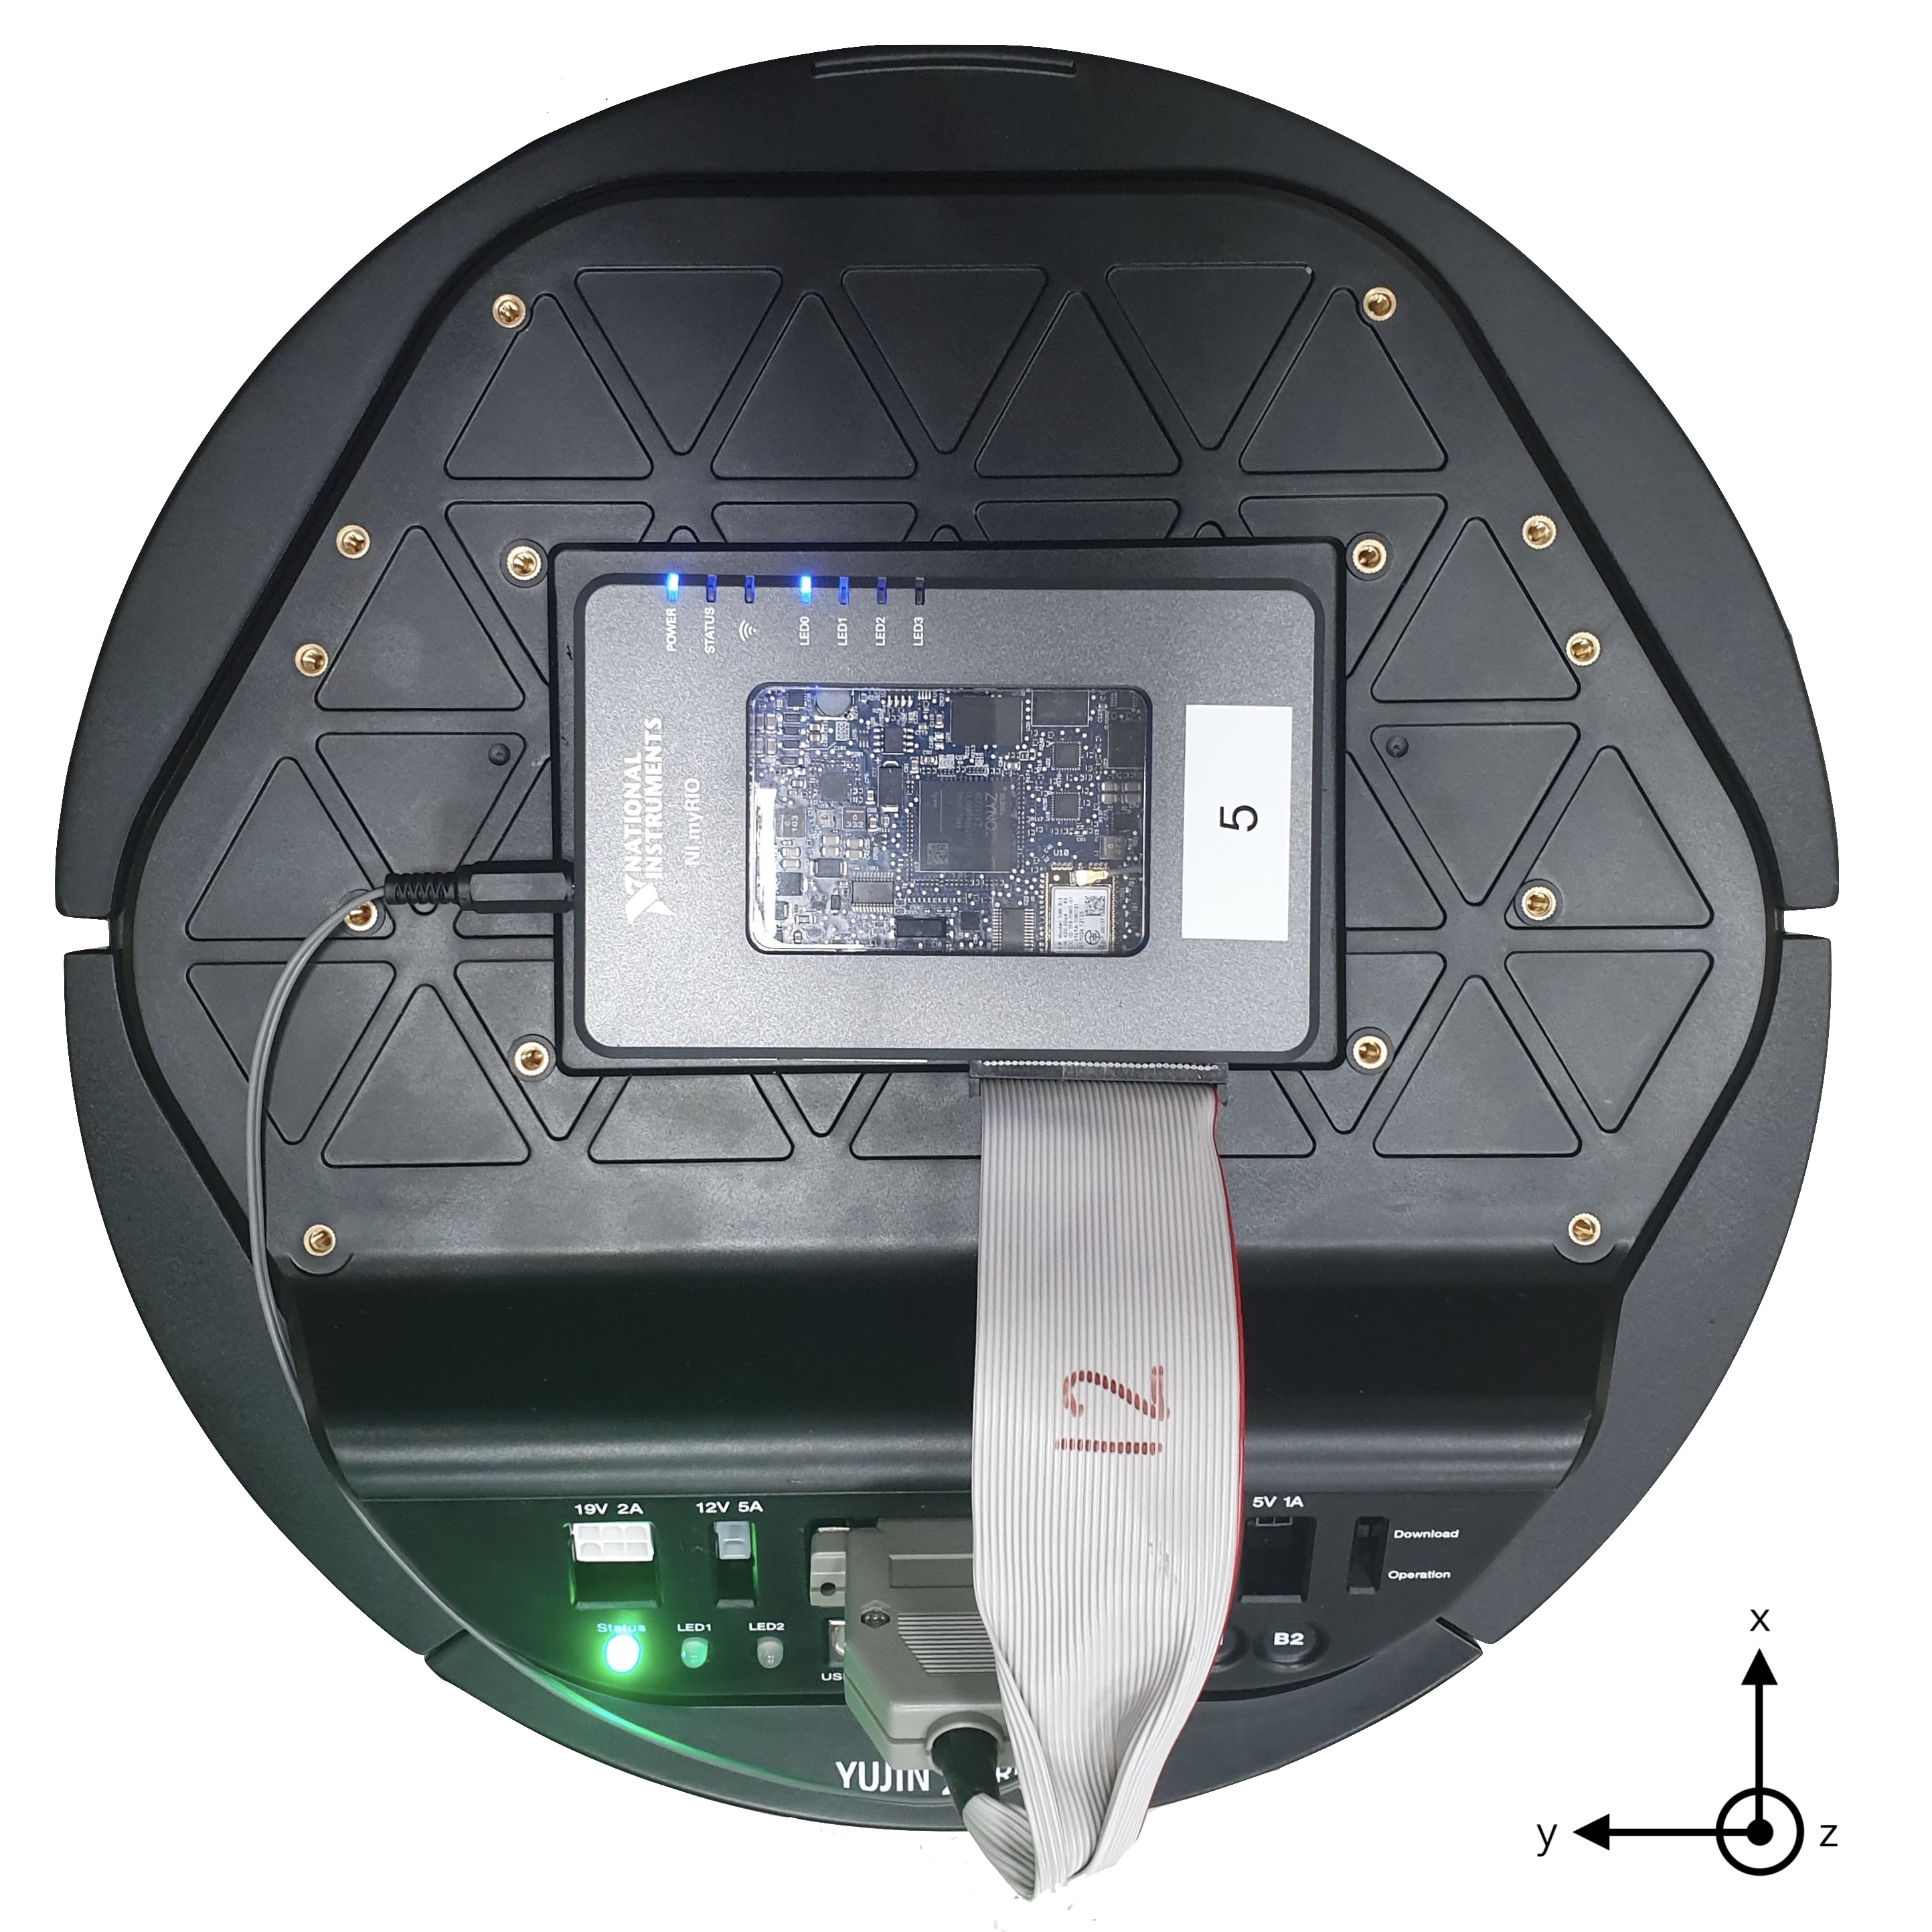
\includegraphics[width=8cm]{Images/Kobuki.png}
    \caption{30cm diameter Kobuki with connected myRIO in bird's eye view}
    \label{fig:kobuki}
\end{figure}

\subsection{Project Requirements}\label{sec:requirements}
To successfully complete the obstacle course, we must follow the following requirements and rules:
\begin{itemize}
    \item \textbf{Play/Pause}: 
    The Kobuki's action will be determined by it's 'B0' button. The robot shall only start when B0 is pressed. When pressed again all movement should be paused and the robot will resume upon another press of B0. The B0 button can also be referred to as the 'Play' button.
    \item \textbf{Driving}:
    The robot should stay level on the ground whilst moving at all times. The original positive $x$ axis position of the Kobuki at the start of the obstacle course determines the 'Ground Orientation', which the Kobuki should always follow. The ground orientation can only change after a power cycle, reprogram or restart of the robot or its embedded controller. There are also additional challenges to overcome whilst driving:
    \begin{itemize}
        \item \textbf{Obstacle Avoidance}:
        The Kobuki should always avoid obstacles in the form of cliffs, wheel hazards, and objects whilst driving even during simultaneous or shortly successive encounters. After encountering obstacles, the Kobuki must be able to reorient and resume driving in ground orientation. The Kobuki is allowed to touch objects as long as it changes course immediately to avoid the obstacle. 
        \item \textbf{Hill Climb}:
        The Kobuki must be able to climb up a hill, drive through the plateau and descend to a final stop on flat ground within 40cm of the bottom of the hill. The robot must be able to orient itself on the hill to execute an orthogonal climb or descent. At any time the robot must not go over the edge of the hill.
    \end{itemize}
    \item \textbf{Performance Specfications}
    \begin{itemize}
        \item \textbf{Rotation}: The Kobuki should not rotate more than 180 degrees.
        \item \textbf{Chattering}: Chattering and erratic movement should not be exhibited.
        \item \textbf{Abnormal Termination}: With the exception of power or mechanical failure, the robot should not stop at any time.
        \item \textbf{Obstacle Hugging}: The Kobuki is not allowed to repeated encounter the same obstacle for navigation.
        \item \textbf{Timeliness}: The obstacle course should be completed within 180 seconds.
    \end{itemize}
\end{itemize}
\section{System Analysis}\label{sec:system}
\vspace{-0.2cm} Sensors and actuators are hardware elements that govern the execution of cyber-physical systems in terms of how well it performs and what it is capable of. Understanding the limitations in hardware is a key step to designing systems that efficiently meet specifications. In addition, to enable smarter controller design, whilst analysing the physical Kobuki, comparisons were also drawn with the simulation environment, which is based on a physical model that simulates rigid body dynamics and render them in 3D \cite[p.~30]{labguide}.

\subsection{Kobuki Sensors and Actuators}
%A basic description of the sensor data available to myRIO and how it was used in your algorithm
\vspace{-0.2cm} With a variety of sensors available on the Kobuki as shown in Figure \ref{fig:kobuki_sensors}, we chose to use applicable sensors for our obstacle navigation. Table \ref{table:kobuki_sensors} shows the sensors we used in our design and the obstacle course specifications that the sensors will help achieve. The wheel drop sensors and bumpers are both triggered as boolean outputs when the requirement of the wheel touching the ground or bumper uncollided is no longer true. The cliff sensor will avoid cliffs deeper than 5cm \cite{kobuki_datasheet}, the sensor range is 2 - 15cm \cite{kobukisensors}.
\begin{figure}[H]
    \centering
    \includegraphics[width=12cm]{Images/kobuki_spec.jpg}
    \caption{Angle view of Kobuki with sensors labelled \cite{kobuki_spec_pic}}
    \label{fig:kobuki_sensors}
\end{figure}
\begin{table}[H]
\begin{center}
\begin{tabular}{ |l|c|c|c| } 
    \hline
    \textbf{Sensor} & \textbf{Number} & \textbf{Target Specification} & \textbf{Output} \\ 
    \hline
    Wheel Drop Sensor & 2 (left, right) & Maintain ground contact & Boolean\\
    \hline
    Cliff Sensor & 3 (left, center, right) & Hill climb edge avoidance & Boolean and Raw\\
    \hline
    Bumper & 3 (left, center, right) & Object avoidance & Boolean\\
    \hline
\end{tabular}
\caption{Kobuki Sensors} \label{table:kobuki_sensors}
\end{center}
\end{table}
\vspace{-0.5cm}
The Kobuki polls the sensors at 50Hz and returns the above sensor data as default ``Basic Sensor Data" in the form of a hexadecimal bytestream \cite{kobukisensors}. These sensors were also available on the simulation robot model. In addition to direct sensor data, the Kobuki also receives information on distance travelled (in mm) and angle rotated (in degrees) since origin. Compared to the simulation output, the real distance is signed and has angles unwrapped within $(-180^\circ, 180^\circ)$. The distance travelled is derived from the wheel movement so if the wheels were slipping, the reported distance travelled will still increase. The simulation only records the actual distance moved by the robot \cite[p.~37]{labguide}. The maximum rotational velocity is $180^\circ$/s (anything above $110^\circ$ will see degraded gyro performance) and the maximum translational velocity is 70cm/s \cite{kobuki_datasheet}. 

\subsection{Accelerometer ADXL330} \label{sec:acc}
\vspace{-0.2cm} In order to detect inclination and reorient the Kobuki on an incline, we used the accelerometer on the myRIO instead of the Kobuki gyroscope that is already used for determining rotation. The accelerometer offers a greater precision for readings in 3 axes ($x$, $y$, $z$) in comparison to the gyroscope's single axis reading. This will allow a greater sensitivity to the ground's incline environment. The accelerometer used in myRIO is the ADXL330 supplied by Analog Devices. It is also used in the Wiimote, which we used to experiment with the nature of accelerometer data. Figure \ref{fig:ADXL330} shows the pin configuration of the accelerometer and the respective axis orientations, which is rotated $180^\circ$ on the Kobuki to align the drive direction with $+x$.
\begin{figure}[H]
    \centering
    \includegraphics[width=4cm]{Images/ADXL330.png}
    \caption{Pin Configuration of ADXL330 \cite{ADXL330}}
    \label{fig:ADXL330}
\end{figure}

\vspace{-0.2cm} \noindent Using the accelerometer readings we calculate the pitch $(\theta)$ and yaw $(\psi)$ angles in radians with respect to the Kobuki axis orientation in Figure \ref{fig:kobuki} \cite{fisher_2011}.
Figures \ref{fig:pitch} and \ref{fig:yaw} indicate the angles in context of the Kobuki with both pitch and yaw angles showing increasing positive values. The resulting angle expressions in Eq.\ref{eq:accel_pitch} and Eq.\ref{eq:accel_yaw} are adapted from Fisher \cite{fisher_2011}. Note the yaw angle's arctan argument used in Eq.\ref{eq:accel_yaw} is defined instead of $\frac{x}{y}$ from Fisher \cite{fisher_2011}. Instead this argument is used to generate the same yaw behaviour in simulation as the myRIO mounting on the model has the $\pm x$, $\pm y$ and $\pm z$ axes swapped \cite[p.~235]{labguide}.
\begin{align}
    \theta &= \arccos \biggr( \frac{z}{\sqrt{x^2 + y^2 + z^2}} \biggr)\label{eq:accel_pitch}\\
    \psi &= \arctan(-\frac{y}{x})\label{eq:accel_yaw}
\end{align}
\vspace{-0.2cm}
\begin{figure}[H]
    \centering
    \begin{minipage}{0.45\textwidth}
    \centering
    \vspace{1cm}
    \includegraphics[width=3cm]{Images/Pitch.png}
    \caption{Positive pitch angle from 0, increasing in the direction of +z}
    \label{fig:pitch}
    \end{minipage}%
    \hspace{0.5cm}
    \begin{minipage}{0.45\textwidth}
    \centering
    \includegraphics[width=2.2cm]{Images/Yaw.png}
    \caption{Positive yaw angle from 0, increasing in the direction of -y}
    \label{fig:yaw}
    \end{minipage}
\end{figure}

\subsubsection{Tuning Accelerometer Readings}\label{sec:accelerometer_LPF}
\vspace{-0.2cm} The typical output range for the accelerometer is $\pm 3.6g$ with a typical output voltage bias of 1.5V at 0$g$ and typical sensitivity of 300mV/$g$ for an operating range of 1.8 - 3.6V \cite{ADXL330}. The digital output received by the device will be $f(x) = 0.3x + 1.5$, rearranging this we get $x$ as the accelerometer reading in $g$,
\begin{align}
    x = \frac{f(x) - 1.5}{0.3}
\end{align}
With the level of sensitivity and fast sensor response rate, the accelerometer readings vary too frequently and may result in instability of robot performance. Therefore, we needed to use a low pass filter to average out the accelerometer reading so that it is accurate enough to represent the current state but also smooths out peak readings and avoids sensory overload. A discrete time solution would be ideal to implement on the digital system. A solution used in Ozyagcilar's paper was the exponential low pass filter, where the discrete time frequency transfer function is expressed in Eq.\ref{eq:LPF_freq} \cite[p.~16]{ozyagcilar}. It has a single pole on the real axis at $1 - \alpha$, where $\alpha$ represents the filter coefficient and should be smaller than 1 to keep the pole within the unit circle thereby guaranteeing system stability. 
\begin{align}
    H(z) &= \frac{\alpha}{1 - (1 -\alpha)z^{-1}}\label{eq:LPF_freq}
\end{align}
Expressing Eq.\ref{eq:LPF_freq} in the discrete time domain gives $y[n] = (1 - \alpha) y[n - 1] + \alpha x[n]$ \cite[p.~16]{ozyagcilar}. The difference equations describes the filter taking in a portion of the previous accelerometer reading and adding it to a corresponding proportion of the current reading. The filter would be used for each axis' reading independently before the smoothed output is used in Eq.\ref{eq:accel_pitch} and Eq.\ref{eq:accel_yaw} to calculate the pitch and yaw angles. The value of $\alpha$ was determined through experimentation on the live system.
\section{Design Methodology}\label{sec:design}
%% methodology behind how we decided to tackle hill climb and obstacle avoidance
% flowchart here?
\vspace{-0.2cm} Exploring the complexity introduced by an unknown obstacle course led us to abstract key system features via variables and layers and hence designing an Hierarchical Extended Finite State Machine (HFSM). Navigating the obstacle course using a HFSM allows flexibility in control and a level of autonomous decision making by the robot in response to sensor and actuator signals. The two main design challenges of obstacle avoidance and hill climbing were approached separately to simplify the design process. Simulation of the algorithms were used to fine tune the design via CyberSim. The play/pause states were adopted from the templates provided and were tested for feasibility. Overall it was an iterative process going between analysis/design, simulation and deloying/testing. Figure \ref{fig:workflow} depicts the workflow adopted in the design process. The details of implementation, simulation and how we used the Kobuki for testing will be discussed in Section \ref{sec:testing}.
\begin{figure}[H]
    \centering
    \includegraphics[width=16cm]{Images/Workflow.png}
    \caption{Design workflow \cite[p.~36]{labguide}}
    \label{fig:workflow}
\end{figure}

\clearpage
\subsection{Obstacle Avoidance}\label{sec:obstacle_alg}
\vspace{-0.2cm} The obstacle avoidance algorithm was designed gradually through iteration. Each development cycle introduced new use cases and targeted problems from the previous round. %%% figures of basic FSM required here?
\begin{enumerate}
    \item A minimum viable product (MVP) version of a state machine used for obstacle avoidance was implemented. When the Kobuki collided with an object it would reverse, rotate $90^\circ$ right, travel parallel to the collision point, rotate back into the original line of travel and continue.\\
    \textbf{Success}: This algorithm proved effective at travelling around a single obstacle.\\
    \textbf{Issues}: The Kobuki only rotates right whilst avoiding the obstacle, which means if the right bumper was triggered it would have to a long way around as shown in Figure \ref{fig:Obstacle1}.
    \item The algorithm was improved by rotating the Kobuki away from the obstacle - in the direction opposite to the bumper sensor that was triggered. If the right bumper was pressed then the Kobuki would avoid by rotating left and vice versa. If the centre bumper was pressed, it remains rotating right.\\
    \textbf{Success}: This algorithm proved to be much more efficient at avoiding obstacles by taking a shorter path responding with respect to each sensor.\\
    \textbf{Issues}: If the Kobuki hit an obstacle during the avoiding state it would reverse, rotate and avoid again as seen in Figure \ref{fig:Obstacle2}. This loses the ground orientation and does not meet design requirements.
    \begin{figure}[H]
    \centering
    \begin{minipage}{0.45\textwidth}
        \centering
        \vspace{0.5cm}
        \includegraphics[width=4.6cm]{Images/Obstacle1.png}
        \caption{Inefficient path around an obstacle when the avoidance rotation is solely rotate $90^\circ$ right}
        \label{fig:Obstacle1}
    \end{minipage}%
    \hspace{0.5cm}
    \begin{minipage}{0.45\textwidth}
    \centering
        \includegraphics[width=8cm]{Images/Obstacle2.png}
        \caption{Going in the opposite direction to original drive after responding to a second obstacle whilst avoiding the first}
        \label{fig:Obstacle2}
    \end{minipage}
    \end{figure}
    \item The final iteration handled meeting obstacles during the avoiding state. A new state was added to ensure that the Kobuki would rotate back to the ground orientation after the second reverse. Additionally, to avoid getting stuck by rotating back and forth between obstacles, a variable was added to change the direction that the Kobuki turned when the centre bumper was pressed. For example, after the first corner situation the centre bumper would now trigger a left rotate instead of right rotate in avoidance.
    \begin{figure}[H]
        \centering
        \includegraphics[width=6cm]{Images/Obstacle3.png}
        \caption{Orange arrows show the path after encountering an object whilst in an obstacle avoiding state}
        \label{fig:Obstacle3}
    \end{figure}
\end{enumerate}

\subsection{Hill Climb}\label{sec:hill_alg}
\vspace{-0.2cm} The hill climbing algorithm also went through design iterations for detecting an incline and reorienting to travel directly uphill or downhill. The hill is assumed to slope along one axis only in the obstacle course. However, slope testing in the simulation presented difficulties and are discussed in Section \ref{sec:cybersim}.
\begin{enumerate}
    \item The MVP algorithm used the low pass filtered accelerometer readings in $g$ to detect a hill (see Section \ref{sec:accelerometer_LPF}). An incline was detected when the absolute value of the $z$ accelerometer decreased below a  threshold from $1g$. When on a hill, the Kobuki rotated until the absolute value of the $y$ accelerometer increased beyond a threshold above $0g$.\\
    \textbf{Success}: The algorithm proved responsive to pitch detection for an incline.\\
    \textbf{Issues}: Reorientation was difficult with the accelerometer value from just the $y$ axis as it was too sensitive to fluctuations and wasn't indicating the orientation correctly.
    
    \item Equations in Section \ref{sec:acc} were used to calculate pitch and yaw angles via the accelerometer. Additionally, when the Kobuki is first unpaused $x$, $y$, and $z$ values were set to zero to avoid calibration bias.\\
    \textbf{Success}: Hill detection and hill orientation performance was greatly improved. The reliability of detection improved with the zero initialisation.\\
    \textbf{Issues}: Thresholds set for both pitch and yaw angles for hill orientation showed significant chattering.
    
    \item The final iteration radically changed the way the Kobuki reoriented on a hill. Instead of stopping and rotating until a threshold is met, a feedback loop was introduced. The relative speeds of each wheel were adjusted to be proportional to the difference between the current orientation and the desired orientation. This is shown in Figure \ref{fig:hillARC} in comparison with the chattering path.
    \begin{figure}[H]
        \centering
        \includegraphics[width=6cm]{Images/ChatterVSArc.png}
        \vspace{-0.2cm}
        \caption{Left: Reorienting path with chattering; Right: Reorienting path with rotation angle feedback}
        \label{fig:hillARC}
    \end{figure}
\end{enumerate}

\subsection{Hierarchical Extended Finite State Machine}\label{sec:FSM}
%A complete FSM diagram (including pause states) of the robot algorithm using the notation covered in the lectures. If you use an Extended state machine, or state refinements, you must show all states, variables and transitions.
\vspace{-0.2cm} There are 3 levels to the final hierarchical extended finite state machine. The run/pause level, the obstacle avoidance level and the hill climbing level. When the system is in the run state, the system enters the state refinement for obstacle avoidance. During the drive state of the obstacle avoidance refinement the system enters another state refinement to handle hill climbing. Note that the transitions to the states with refinements are history transitions - the refinements remember which state they are in rather than resetting. This is crucial for the pause behaviour and for tracking the hill states. This design neatly abstracts the different tasks that the Kobuki must perform. There is also the added benefit of being able to avoid obstacles while hill climbing - no additional states are required to avoid cliffs. The state diagram is shown in Figure \ref{fig:FSM}. Trigger and action labels are used to simplify the diagram, see Tables \ref{tab:triggers} and \ref{tab:actions} for the label definitions. The output converter in Table \ref{tab:outputs} uses the variable \textit{DriveMode} to convert to the left and right wheel speeds on each update. The \textit{incline} and \textit{tiltAngle} variables are calculated on each update according to the pitch and yaw calculations of Section \ref{sec:acc}. % consider flowchart?

\begin{figure}[p]
    \centering
    \begin{tabular}{ll}
      \textbf{inputs:}   & \textit{B0} : pure\\
                         & \textit{cliffLeft, cliffCentre, cliffRight} : pure \\
                         & \textit{bumpLeft, bumpCenter, bumpRight} : pure \\
                         & \textit{wheelDropLeft, wheelDropRight} : pure\\
                         & acc : $\mathbb{R}^3$\\
                         & \textit{netAngle, netDistance} : $\mathbb{R}$\\
      \textbf{variables:}& \textit{driveMode} : \{FORWARD, BACKWARD, ROTATE\_LEFT, ROTATE\_RIGHT, ARC, STOP\}\\
                         & \textit{incline, tiltAngle} : $\mathbb{R}$\\
                         & \textit{turnPct} : $\mathbb{R}$\\
                         & \textit{distance, angle} : $\mathbb{R}$\\
                         & \textit{obstacleLoc} : \{LEFT, CENTRE, RIGHT\}\\
                         & \textit{offsets} : $\mathbb{R}^3$\\
                         & \textit{centreTurn} : \{\textit{true, false}\}\\
     \textbf{outputs:}   & \textit{leftWheelSpeed}, \textit{rightWheelSpeed} :  $\mathbb{R}$\\
    \end{tabular}
    \includegraphics[width=\textwidth]{Images/Finite_State_Machine_v2.png}
    \caption{Extended State Machine (See Tables \ref{tab:triggers} and \ref{tab:actions} for Trigger and Action definitions)}
    \label{fig:FSM}
\end{figure}

\begin{table}[p]
    \centering
    \begin{tabular}{|c|c|}
        \hline
        Name        & Trigger Definition \\
        \hline\hline
        PauseButtonPressed & \textit{B0} \\
        \hline
        PauseButtonReleased    & $\neg$\textit{B0}  \\
        \hline
        ObstacleDetectedLeft & \textit{cliffLeft} $\lor$ \textit{bumpLeft} $\lor$ \textit{wheelDropLeft}\\
        \hline
        ObstacleDetectedRight & \textit{cliffRight} $\lor$ \textit{bumpRight} $\lor$ \textit{wheelDropRight}\\
        \hline
        ObstacleDetectedCentre & \textit{cliffCentre} $\lor$ \textit{bumpCentre}\\
        \hline
        ObstacleDetected & ObstacleDetectedLeft $\lor$ ObstacleDetectedRight $\lor$ ObstacleDetectedCentre\\
        \hline
        DistanceReached & abs(\textit{netDistance} - \textit{distance}) $\geq$ distanceReachedThreshold\\
        \hline
        DistanceReachedLeft & DistanceReached $\land$ (\textit{obstacleLoc} = LEFT $\lor$ \textit{centreTurn})\\
        \hline
        DistanceReachedRight & DistanceReached $\land$ $\neg$(\textit{obstacleLoc} = LEFT $\lor$ \textit{centreTurn})\\
        \hline
        DistanceReachedReverse & abs(\textit{netDistance} - \textit{distance}) $\geq$ distanceReachedReverseThreshold\\
        \hline
        DistanceReachedReverseLeft & DistanceReachedReverse $\land$ (\textit{obstacleLoc} = LEFT $\lor$ \textit{centreTurn})\\
        \hline
        DistanceReachedReverseRight & DistanceReachedReverse $\land$ $\neg$(\textit{obstacleLoc} = LEFT $\lor$ \textit{centreTurn})\\
        \hline
        AngleReached & abs(\textit{netAngle} - \textit{angle}) $\geq$ 90\\
        \hline
        FlatDetected & abs(\textit{incline)} $<$ flatDetectedThreshold\\
        \hline
        InclineDetected & abs(\textit{incline}) $>$ inclineDetectedThreshold\\
        \hline
    \end{tabular}
    \caption{Trigger Definitions}
    \label{tab:triggers}
\end{table}

\begin{table}[p]
    \centering
    \begin{tabular}{|c|c|}
        \hline
        Name        & Action Definition \\
        \hline\hline
        SetObstacleLocLeft & \textit{obstacleLoc} := LEFT \\
        \hline
        SetObstacleLocRight & \textit{obstacleLoc} := RIGHT \\
        \hline
        SetObstacleLocCentre & \textit{obstacleLoc} := CENTRE \\
        \hline
        ResetDistance & \textit{distance} := \textit{netDistance}\\
        \hline
        ResetAngle & \textit{angle} := \textit{netAngle}\\
        \hline
        Forward & \textit{driveMode} := FORWARD \\
        \hline
        Reverse & \textit{driveMode} := BACKWARD \\
        \hline
        RotateRight & \textit{driveMode} := ROTATE\_RIGHT \\
        \hline
        RotateLeft & \textit{driveMode} := ROTATE\_LEFT \\
        \hline
        Stop & \textit{driveMode} := STOP \\
        \hline
        Arc & \textit{driveMode} := ARC \\
        \hline
        AscendHill & \textit{turnPct} := $-\textit{tiltAngle}/\pi$\\
        \hline
        DescendHill & \textit{turnPct} := $-(\textit{tiltAngle}-\text{sign(\textit{tiltAngle})}\pi)/\pi$\\
        \hline
        ToggleCentreTurn & \textit{centreTurn} := $\neg$ \textit{centreTurn}\\
        \hline
        SetOffsets & \textit{offsets}:= \{\textit{acc.x}, \textit{acc.y}, $1.0-\textit{acc.z}$\}\\
        \hline
    \end{tabular}
    \caption{Action Definitions}
    \label{tab:actions}
\end{table}

\begin{table}[p]
    \centering
    \begin{tabular}{|c|c|c|}
        \hline
        \textit{DriveMode}  & \textit{leftWheelSpeed} & \textit{rightWheelSpeed} \\
        \hline\hline
        FORWARD & SPEED & SPEED \\
        \hline
        BACKWARD & $-$SPEED & $-$SPEED \\
        \hline
        ROTATE\_LEFT & $-$SPEED & SPEED \\
        \hline
        ROTATE\_RIGHT & SPEED & $-$SPEED \\
        \hline
        ARC & $\text{SPEED}(1.0-\textit{turnPct})$ & $\text{SPEED}(1.0+\textit{turnPct})$ \\
        \hline
        STOP & 0 & 0\\
        \hline
    \end{tabular}
    \caption{Output Converter}
    \label{tab:outputs}
\end{table}

% I feel like we need to discuss more here?
% describe key states? 
% how many states, efficiency etc... 
% why we decided on hierarchical
\newpage
\section{Implementation and Testing}\label{sec:testing}
Briefly alluded to in Section \ref{sec:system}, the simulation environment CyberSim is based on a SolidWorks modelling the rigid body dynamics of the Kobuki. The LabVIEW Robotics Environment Simulator solves ordinary differential equations (ODEs) for the dynamics of the system and renders the outcome into a display dialogue in 3D \cite{labguide}. Our envisioned state machine as mentioned in Section \ref{sec:FSM}, came to it's final states through multiple iterations. Regular testing of each design phase on the physical Kobuki brought our attention to issues that weren't obvious in theoretical planning or simulation.

\subsection{LabView vs. Microsoft Visual Studio (C/C++) and Eclipse}
\vspace{-0.2cm} LabView is the system engineering software produced by National Instruments to run the Kobuki obstacle course lab exercises. It provides a graphics user interface (GUI) approach to allow the user to drag and drop `blocks' into project surfaces and program visually. Microsoft Visual Studio (VS) is a standard integration development environment (IDE) that's used across the workplace for code development. The IDE comes with inbuilt compilers and debugger along with other software engineering basics such as automatic indentation and variable searching to ease coding. To run the code on the Kobuki, it would need to be transferred over into an Eclipse project file in order to connect to the Kobuki hardware. Both options allow simulation running CyberSim when the associated LabView software development kit (SDK) was downloaded and available.\\

To understand both implementation options better, the first MVP algorithm for obstacle avoidance was programmed using both LabView and VS/Eclipse. Figure \ref{fig:LabView} shows the CyberSim output indicating the state on a LabView state chart and Figure \ref{fig:VS} shows Visual Studio during a debugging session. To summarise this initial experiment, Table \ref{tab:labviewVSC} shows the key unique positives and negatives of both tools (comparison was made so that the negatives in one tool doesn't have a corresponding positive in the other tool). Clearly shown, VS and Eclipse offered more positives and less negatives than LabView. The unsolved reason to why the left bumper block wasn't usable in LabView was also a key reason why it was not chosen - without the left bumper sensor the Kobuki would fail to meet obstacle avoidance requirements when encountering any left obstacle. The main negative from Eclipse was the timeout, which was avoided by a ``TF" timeout override block in LabView. In week 10, the demonstrators shared the solution of writing \texttt{nohup} to override the TCP timeout before the binary execution on the Kobuki. In addition, instructions for wifi connection to the Kobuki was also given, which allowed faster testing and sharing of iterated code via local machine and GitHub repositories. Thence, the chosen implementation tool was Visual Studio and Eclipse.
\begin{figure}[H]
    \centering
    \begin{minipage}{0.45\textwidth}
    \centering
    \includegraphics[width=8cm]{Images/LabViewStateChart.png}
    \caption{LabView statechart present in CyberSim for iRobot \cite[p.~32]{labguide}}
    \label{fig:LabView}
    \end{minipage} \hspace{0.5cm}% 
    \begin{minipage}{0.45\textwidth}
    \centering
    \includegraphics[width=8cm]{Images/VisualStudio.png}
    \caption{Visual Studio IDE connected to GitHub for source control for the project \texttt{libstatechart.sln}}
    \label{fig:VS}
    \end{minipage}
\end{figure}

\begin{table}[!ht]
    \centering
    \begin{tabularx}{\textwidth}{|X|X|}
        \hline
        \textbf{LabView} & \textbf{Visual Studio/Eclipse (C/C++)}\\
        \hline
        \begin{itemize}
            \item[+] Easy to visualise states and transitions
            \item[+] Code deployment onto Kobuki was very simple, it required only the single download button
            \item[+] CyberSim can show the states that the simulation traverses, thus allowing simple debugging
            \item[-] The LabView platform was often unstable and crashed three times unexpectedly without saving
            \item[-] Iteration of code was difficult to track all the different transition blocks that required to change
            \item[-] The GUI was not user friendly and was time consuming to individually select blocks and made sure lines fully connected
            \item[-] The use of variables wasn't very intuitive and required a lot of extra handling to initialise the variable abd add it individually to each transition
            \item[-] Repeated transitions or actions couldn't easily be reused and looks very convoluted
            \item[-] The Kobuki we used had a disabled left bumper which wasn't able to be controlled
            \item[-] Program was only accessible in the workshop sessions on the computers with LabView
        \end{itemize}
        &
        \begin{itemize}
            \item[+] Encouraged collaboration via GitHub to share the code and track changes or revert to previous versions when required
            \item[+] Debugging was very straightforward with standard error messages from the C compiler
            \item[+] Code written could include comments that described the process and provided more context behind the program
            \item[+] C offered execution efficiency with the variety of intuitive functions included in standard libraries and sped up the programming
            \item[+] All team members are experienced with coding in C and working on source code allowed contribution from both Windows and Mac users
            \item[-] Deployment on the Kobuki required a lot more steps to connect to a remote target, generate a binary and replace the original binary in the path and then execute via a terminal
            \item[-] Deployment on the Kobuki communicates using the TCP protocol and has a timeout
            \item[-] Configuration in Eclipse requires fiddly setup that may require starting from scratch if the machine is not already set up correctly
        \end{itemize}\\
        \hline
    \end{tabularx}
    \caption{Positives and negatives of LabView and Visual Studio/Eclipse}
    \label{tab:labviewVSC}
\end{table}

\subsection{Building a State Machine in C}
\vspace{-0.2cm} There are many ways to implement a state machine using C. There was a risk of having unmanageable and unreadable spaghetti code filled with conditional statements \cite{codingFSM}. The problem with using a conditional statement approach is the difficulty of seeing the difference between states, variables, triggers and actions as each state may require its independent variables to activate triggers and actions to capture dynamic history. A better approach defined states as structs and triggers/actions as function pointers \cite{structs_fnc_ptrs}. This means the main function only needs to look at the current state, check the triggers from the state and if any trigger returns true, perform the actions of that transition.\\

Once the core logic was implemented then adding states was as simple as creating a struct with function pointers to describe transitions. Functions that were commonly used such as calculating angles or checking for angle rotated were easily reused. Pointers offered a lot of flexibility in code development especially when iterating through new and uncertain approaches, such as how we were assessing the angles. An entire state only needed to change where the action pointed to if a new approach was tested in a new function without affecting other transitions. Furthermore, hierarchical state machines were easily implemented by allowing each state to contain another state. In practice, each refinement from the design (see Section \ref{sec:FSM}) was wrapped in a `controller' to handle the variables and behaviour (see Appendix \ref{app:code} to view source code).\\

Conditional statements were initially used for the MVP algorithm for obstacle avoidance, however, as complexity grew a new Git branch was created to use structs. Eventually the implementation proved so much easier and versatile that the structs branch was squash merged and replaced the original code. An example shown in Figures \ref{fig:DriveAvoidIfs}-\ref{fig:DriveAvoidStructs} compares the effort required between using switch case/conditional statements and structs/function pointers for implementing the extra \textit{ReverseCorner} state from the \textit{DriveAvoid} state. This was our third iteration for developing the obstacle avoidance algorithm in Section \ref{sec:obstacle_alg}. Blue indicates what's already present in the obstacle avoidance, yellow shows reused functions, three Figure \ref{fig:DriveAvoidStructs} there are only a total of three states at the end of the implementation and reusing existing functions was easy by swapping the left and right functions being pointed to. The end of the if statement changes in Figure \ref{fig:DriveAvoidIfs} shows little connection to what was used already and shows a total of five states with overlapping behaviours to the original code for \texttt{DriveAvoid}. What continues after the two new \textit{CornerTurn} states are also be even more nested in if statements.\\
\begin{figure}[H]
    \centering
    \includegraphics[width=12cm]{Images/DriveAvoidIfs.png}
    \caption{Flowchart describing three new if conditions and two new states added to existing conditional statements}
    \label{fig:DriveAvoidIfs}
\end{figure}
\begin{figure}[H]
    \centering
    \includegraphics[width=11cm]{Images/DriveAvoidStruct.png}
    \caption{Flowchart describing one new function and one new state added to existing transitions}
    \label{fig:DriveAvoidStructs}
\end{figure}

% Simulation results, and how the simulation was shit.
\subsection{Simulation using CyberSim}\label{sec:cybersim}
\vspace{-0.2cm} The simulation environment determines noise behaviours through random numbers, which means that each Kobuki test trace will never be exactly the same. Being non deterministic is beneficial when testing as it better emulates a real world situation as environmental factors that influence outcomes will always change \cite{labguide}.\\

CyberSim was helpful in testing obstacle avoidance and the development iterations concluded with satisfactory results. The ability to increase speeds to simulate the robot faster was useful sometimes e.g. when quickly testing the change for different bumpers leading to different turn directions. The \texttt{Navigation Maze} environments were very effective in testing the \textit{ReverseCorner} state in the last development iteration. The first try successfully demonstrated the robot turning around the opposite way from the second obstacle but when hitting the centre bumper again the turning direction (initially \texttt{centreTurn = false} and will turn left) did not change although the function \texttt{ToggleCentreTurn()} had reset the variable (when encountering an obstacle during \textit{DriveAvoid}, \texttt{centreTurn = true} and will turn right). Troubleshooting this concluded that system variables were always reset to the initial default upon state change despite the function being executed. This was a flaw in the implementation of the core hierarchical extended state machine system. The solution was to make the \texttt{centreTurn} variable a global variable to override the reset and this worked in simulation.\\ 

Despite successes in obstacle avoidance, CyberSim was not the best simulation environment for hill climb. Some key issues with the solutions or alternative tests are expressed in Table \ref{tab:cybersim_hillclimb} and Figure \ref{fig:cybersim_hillclimb} shows the Kobuki in CyberSim whilst on an incline in \texttt{Environment - south ramp left}. Through what was successfully simulated in CyberSim, a key conclusion was that the hill climb MVP algorithm, which used raw accelerometer angles to detect incline and reorient directly towards uphill and downhill, did not produce reliable behaviours. This therefore led to the second iteration, which used angle calculation from the accelerometer readings (see Section \ref{sec:hill_alg}). Testing this in CyberSim saw the robot detecting and reorienting being less affected by accelerometer reading fluctuations.
\begin{table}[H]
\centering
\begin{tabularx}{\textwidth}{|X|X|}
    \hline
    \textbf{Key Issue in CyberSim Hill Climb} & \textbf{Solution or Alternative Tests}\\
    \hline
    The slope on simulation environments e.g. \texttt{Environment - south ramp left}, is not tilted via a single axis and there wasn't a clear way to visually confirm whether the robot was driving directly uphill or downhill. 
    & 
    Meticulous observation of the thresholds and angles with used to calibrate the testing. Implementation on the physical Kobuki was always used to confirm behaviours.\\
    \hline
    Incline thresholds were different to test ramp used for testing in the workshops. Simulation thresholds were very small and visually there wasn't a good way to tell if the hill climb states were active. The accelerometer readings also suffered a lot from fluctuations, where randomised noise produced non-deterministic confusing outcomes.
    &
    The code included an \texttt{isSimulator} variable to toggle between the real and simulator thresholds. Again, implementation on the physical Kobuki was necessary to confirm incline detection.\\
    \hline
    The Kobuki in simulation had the accelerometer directions swapped for the $\pm y$ and $\pm x$ axis.
    &
    \texttt{isSimulator} also triggered a different yaw angle $\psi$ calculating formula (see Section \ref{sec:acc}).\\
    \hline
    The environment did not offer a plateau to test middle flat state during hill climb.
    & 
    Testing on a plateau in real life was used to confirm Kobuki behaviours.\\
    \hline
    CyberSim does not have the same 'pause' function as the B0 button. Even though the button can be pressed on the GUI, what is outputted is only a simulation pause and overrides any state changes \cite[p.~33]{labguide}.
    &
    The play/pause states were tested on the physical Kobuki whilst testing hill climb. B0 button was pressed to start the Kobuki, pause and unpause it.\\
    \hline
\end{tabularx}
\caption{Issues and Solutions or Alternatives whilst using CyberSim for testing Hill Climb algorithms}
\label{tab:cybersim_hillclimb}
\end{table}
\begin{figure}[H]
    \centering
    \includegraphics[width=14cm]{Images/CyberSimSlope.png}
    \caption{Showing the Kobuki in CyberSim on an incline and the small $x$ and $y$ values}
    \label{fig:cybersim_hillclimb}
\end{figure}

\subsection{Kobuki Testing}\label{sec:hill_test}
\vspace{-0.2cm} When testing the obstacle avoidance algorithms on the Kobuki the realisation was that speed was a factor in the accuracy of turning. The final speed was set to \texttt{200} (mm/s) with the intention to make the Kobuki respond relatively fast to complete the obstacle course on time and remain within an accurate range. The wheeldrop sensors were also debated whether to leave in the algorithm as it seemed to pick up minor lifts and trigger obstacle avoidance states. At the end it was decided that the wheeldrop sensors were to remain in obstacle detection as it was a project requirement that the Kobuki remained touching the ground.\\

Hill climb saw the benefits of slower speed on the ramp as well as higher speeds seemed to drive the wheels a lot more and cause the wheels to lift thereby activating the wheeldrop sensors. Using a separate set of thresholds, the incline detection was tuned to be above 0.2 radians ($11.5^\circ$) to allow significant room for fluctuations. Descending angles were also treated for wrapping the calculated results bewteen $\pm 180^\circ$ as the initial trials showed the Kobuki turning back up when the values remained positive on descent. In the \textit{Descending} state, if the calculated \texttt{angle} was greater than 0, $\pi$ was subtracted, otherwise $\pi$ was added. Testing this in week 10 after wifi connection was enabled allowed the angle values and states to be printed in the Eclipse terminal, which meant spotting the error and seeing the correction was very quick. The Eclipse printed outputs can be seen in Figure \ref{fig:eclipse_output}.\\

A final development was fine tuning the chattering during orientation. Implementing a feedback loop to turn a percentage of the measured offset angle saw the Kobuki glide through the tested inclines smooth without stutter. A full test sequence of state outputs from terminal can be seen in Appendix \ref{app:hill_states}. The terminal outputs indicate the implemented hill climb algorithm being able to achieve incline detection moving from \textit{Drive} to \textit{Ascending} and also detecting cliffs and triggering obstacle avoidance states as well as \textit{Descending} and finishing on flat ground on \textit{End}. Whilst testing hill climb, the state outputs from pausing and unpausing were also successful and are captured in Appendix \ref{app:play_pause_states}.
\begin{figure}[H]
    \centering
    \includegraphics[width=15cm]{Images/eclipse_screenshot.PNG}
    \caption{The real time output showing calculated descent angles (rad) and states in the Eclipse terminal}
    \label{fig:eclipse_output}
\end{figure}
\clearpage
\section{Validation}\label{sec:validation}
% some end thing about our performance after it hits challenge requirements
\vspace{-0.2cm} After 10 weeks of workshops and hard fought open lab workshops, on 21 October 2019, 15:15 the designed algorithms and FSM was put to the final test on a novel obstacle course. The obstacle course was approximately 3m by 5m with a total of seven different obstacles in the area, which funnelled to an uphill ramp, plateau and downhill ramp. The starting and end lines were marked out by tape.

\subsection{Endgame - The Final Run}\label{sec:finalrun}
\vspace{-0.2cm} The Kobuki did not succeed in the final obstacle course. We chose to end the Kobuki around 90 seconds into the run as the robot seemed to have lost it's ground orientation so continuing would not have led it through the course. Because the Kobuki did not reach the hill climb section of the course, this part was not tested. Had we been given the chance to run the robot from the last obstacle and demonstrate hill climb, we are confident that the hill climb algorithm is robust through tests on a similar ramp and will be able to demonstrate project requirements to climb the hill, reorient, detect cliffs and stop after descent within 40cm. The relevant testing and design choices are covered in Section \ref{sec:hill_alg} and Section \ref{sec:hill_test}. Figure \ref{fig:KobukiFinalPath} shows the Kobuki's path through the given obstacle course, note the diagram is not to scale. Red shows the initial path with the centre bumper on default turning left and orange shows the path carried out after encountering the wall as an obstacle during obstacle avoidance. The start and finish lines are in yellow.
\begin{figure}[H]
    \centering
    \includegraphics[width=8cm]{Images/KobukiFinalPath.png}
    \caption{Final obstacle course showing the Kobuki path}
    \label{fig:KobukiFinalPath}
\end{figure}

Analysing the outcome (through repeatedly watching the video taken of the final run), there was a clear point where the behaviour of the Kobuki became unexpected and this is labelled by a purple star in Figure \ref{fig:KobukiFinalPath}. The obstacle avoidance worked as expected, including the corner state sequence via \textit{ReverseCorner} to turn back and exhibit the centre bumper now turning right when triggered. The purple point what where the Kobuki should have reoriented towards the slope in the original ground orientation. However, there was a little hiccup seen in the videos, where the Kobuki was seen to rise. A theory is that it may have triggered the hill climb state \textit{Ascending} even though it's unlikely that the slant was more than $11.5^\circ$. But, indicators that support this theory, include the motion seeming to be more of an arc, which coincides with the reorientation feedback loop we have implemented, and the ground orientation was completely lost. Furthermore, during hill climb, obstacle detection was shown to be possible from our previous testing but after encountering obstacles after the purple star moment, the Kobuki seemed to continuously head bump. A theory to explain this could be that two sensors, both right and centre were bumped at the same time leading to the confusion for which side to turn, where the \texttt{centreTurne = true} leading to turn right and \textit{TurnAway} for the right bumper leads to turn left. However, there was no tangible evidence or state outputs from the final run to analyse the behaviour and conclude with confidence (laptops were not allowed).

%Our Kobuki did not manage to pass the obstacle course. Our Kobuki was doing fine at the beginning, successfully avoid some obstacles. However, when Kobuki is at 'DriveAvoid' state to avoid a obstacle, our Kobuki keep driving straight even the parallel distance has reached. Then our kuboki can not perform any obstacle avoidance action.\\

%After we investigate, there is a possible explanation of why the Kobuki did the wired thing in a 'DriveAvoid' state. The kobuki detected a hill at the start of 'DriveAvoid' state, because the head of the kobuki raised up. The reason could be the bulge on the floor, and the sudden change in speed of the Kobuki is too fast. This can result a relatively large reading in accelerator which can lead to hill detected(Explained in detail in Discussion). According to our FSM diagram in figure 8, the kobuki will go into 'Ascending' state. The kobuki is still on the flat ground, so it will also transit to 'Top' state which will result a Forward output. This may explain that our Kobuki can only drive forward and cannot avoid obstacles anymore.

\subsection{Reachability}
Hierarchical Finite State Machine can make our transitions reusable and more efficient. The overall number of distinct state in the implemented hierarchical FSM is 10. However, it's also more complicated to analyse. The usual way to analyse reachability is by flattening the state machine. This can be quite complex and will eventually lead to state explosion because the size of state machine grows exponentially. For the designed FSM, the maximum number of flattened states can be expressed in big O notation as $O(n^M) = O(6^3) = O(216)$, where $n$ represents the maximum number of states in a single hierarchy and $M$ represents the number of hierarchies \cite{FSM}. With the number of states to flatten, ensuring certainty and not missing out on any trace is a challenge. In Alur and Yannakakis's paper \cite{FSM_reachability} they presented an algorithm to determine the reachability where the input is a hierarchical structure $K$ and a subset $T$, consisting of nodes called the ``target region"\cite{FSM_reachability}. The output from their algorithm given $(K,T)$ is to determine whether $T$ is reachable from the top level entry node - in this project's case, the final state and the hill climb region is $T$ and the overall FSM is $K$. Whilst computing the big O output for reachability may be out of scope for this subject, the final \textit{End} state is eventually reachable from \textit{UnpauseWaitButtonPress}. A simplest trace is presented in Figure \ref{fig:endtrace} as an example with the color change indicating different hierarchies and merged states are transitioned states across hierarchies. Note triggers and actions are left out for simplicity and one can refer to Figure \ref{fig:FSM} for details.
\begin{figure}[H]
    \centering
    \includegraphics[width=11cm]{Images/EndTrace.png}
    \caption{A sample trace for the simplest path from \textit{UnpauseWaitButtonPress} to \textit{End}}
    \label{fig:endtrace}
\end{figure}
% do we need to consider LTL?

\subsection{Reliability} % do we need to talk about other theoretical stuff here?
In theory what could have been shown in the Kobuki final run was the transition from \textit{DriveAvoid} to \textit{Ascending} and this is a reachable path. By analysing the FSM, eventually (when incline conditions are met) the \textit{End} state is also reachable. However, physically it is not possible because the Kobuki would have no way of getting itself to the uphill ramp after losing ground orientation. This was an 'anticlockwise thinking' situation that was not considered when testing the FSM algorithms. If \textit{Run/Drive} was $T$ a target region, it would not be reachable from non-initial nodes in the hill climb hierarchy. To improve reliability, a transition back to the run/drive hierarchy would be necessary if incline detection becomes false. A time threshold must also be present to allow differentiation of the \textit{Top} state, where incline is also not true. More testing of the obstacle sensors over more extreme distances or obstacle situations would have encouraged robustness improvements. Having fine tuned actuation from sensors would mean the system is more reliable.
\section{Discussion}
% refer lectures! 
% talk about improvements
%% write something under this title. Titles should not have no content underneath
\subsection{Using Theory in Practice}
%how you applied knowledge from lecture
When we design our state machine, we tend to add a lot more states which are similar to some other state in our satte machine. This was not a efficient way to design a state machine. So we tried to use a hierarchy structure to make our state machine reusable and more logical. From lecture 11, we learn to build a hierarchical finite state machine with historical transition. By this structure, our Kobuki can perform obstacle avoidance with in a run state, and can also perform a hill climb in a drive state. This structure improves the simplicity and readability of our state machine. %insert lecture 11 as a citation?
% using variables, preemption? maybe?... using LPF to treat sensitivity? L 3/4
\\
\colorbox{yellow}{Probably just try to finish filling page 17}

\clearpage
\subsection{Project Achievements}
% a bunch of stuff about what we did great and awesome and what should inspire other kids to do more of this
\vspace{-0.2cm} A summary of the achieved outcomes in testing/simulation and in the final obstacle course in line with the project requirements (see Section \ref{sec:requirements}) is shown in Table \ref{tab:outcomes}.
\begin{table}[H]
\centering
\begin{tabularx}{\textwidth}{|X|X|X|}
    \hline
    \begin{center}
        \textbf{Expected Outcomes - Requirements} (see Section \ref{sec:requirements})
    \end{center} & 
    \begin{center}
        \textbf{Simulation \& Testing Outcomes} (see Section \ref{sec:testing})
    \end{center} & 
    \begin{center}
        \textbf{Final Run Outcome} \hspace{1cm} (see Section \ref{sec:validation})
    \end{center}\\
    \hline
    \underline{Play/Pause:}
    Kobuki does not run until B0 is pressed.
    When running, Kobuki will be paused when B0 is pressed.
    After a paused state, when B0 is pressed again the Kobuki will resume from the state that it was paused.
    & All requirements were met in testing state outputs can be seen in Appendix \ref{app:play_pause_states}. CyberSim did not offer direct button control for B0 to simulate the play/pause function. 
    & Kobuki did not run until B0 is pressed at the starting line. When B0 was pressed it started the obstacle course. The run was terminated when B0 was pressed to pause the robot.\\
    \hline
    \underline{Obstacle Avoidance:}
    The Kobuki should avoid obstacles (cliffs, wheel hazards and objects) whilst driving.
    After encountering obstacles the Kobuki must reorient and resume driving in ground orientation.
    & Obstacle avoidance was observed in both simulation and Kobuki testing. The algorithm always made sure to \textit{Reverse}, \textit{TurnAway}, \textit{DriveAvoid}, \textit{TurnBack} and \textit{Drive}. Wheel hazards were not observed in simulation. On the Kobuki wheels were only a hazard when the speed was greater than 200mm/s. 
    & The Kobuki successfully avoided three obstacles but only managed to reorient back to ground orientation and drive on with the first two obstacles.
    \\
    \hline
    \underline{Hill Climb:}
    The Kobuki must be able to climb a hill, drive through a plateau, and descend to ground before stopping within 40cm from reaching ground.
    Whilst on an incline the Kobuki must reorient to drive in an orthogonal direction to the slope.
    The Kobuki must avoid cliffs on the incline.
    & All requirements were met in Kobuki testing with the final implemented hill climb algorithm. The state outputs can be seen in Appendix \ref{app:hill_states} going through \textit{Drive}, \textit{Ascending}, \textit{Top}, \textit{Descending} and \textit{End}, as well as, obstacle avoidance states \textit{Reverse}, \textit{TurnAway}, \textit{DriveAvoid}, and \textit{TurnBack}.
    & The Kobuki did not reach the hill climb section of the course and therefore did not get to generate hill climb outcomes.
    \\
    \hline
    \underline{Performance:}
    The Kobuki does not rotate more than $180^\circ$.
    Chattering and erratic movements should not be exhibited.
    Abnormal termination is not to occur.
    The Kobuki is not allowed to repeated encounter an obstacle for navigation.
    The obstacle course should be completed within 180 seconds.
    & Rotation more than $180^\circ$, chattering and erratic movements were not observed during simulation or testing. Abnormal termination via the TCP communication timeout was solved using \texttt{nohup} before executing the FSM. The last two points weren't testable until the final run.
    & We did not observe rotations more than $180^\circ$. During obstacle avoidance there was no chattering, however, there was an erratic rise (see Section \ref{sec:finalrun}). The Kobuki did not terminate until B0 was pressed to pause it. The Kobuki never ran the full 180 seconds.
    \\
    \hline
\end{tabularx}
\caption{A summary of the achieved outcomes in comparison to the project requirements}
\label{tab:outcomes}
\end{table}

\textcolor{blue}{Excellent comparison of the achieved outcomes with the expected outcomes and/or specifications are documented with in-depth discussions which put theory, simulations, and or experiments together. Creative and insightful recommendations for further work. Excellent conclusions.}\\ 
\colorbox{yellow}{I reckon we basically did all that hence referred sections in table.}\\
\colorbox{yellow}{Probably just need 'creative and insightful recos'}

\subsection{Learnings and Improvements}
The low pass filter was not enough to filter out the jumps in the accelerometer values when the Kobuki hits an object and/or changes speed rapidly. Since the hill climbing algorithm was developed and tested separately, there was not extensive testing of the combined algorithm. In reality and in the simulation, there was a risk of the Kobuki entering the `ascendHill' state after bumping into an object. Figure \ref{fig:debug_incline} demonstrates that even in simulation an incline is detected during a collision - the value $0.68$ is well above the thresholds used and is caused by the large $y$ value of $-0.81$. A low pass filter is able to successfully smooth out the sensor noise, however it is unable to filter out large disturbances to the system. A more sophisticated system is required to ensure the rapid acceleration of the Kobuki does not trigger the hill state transitions.
\begin{figure}[H]
    \centering
    \includegraphics[width=0.8\textwidth]{Images/debug_incline}
    \caption{Debugging Simulation during Collision}
    \label{fig:debug_incline}
\end{figure}

In practice the state machine is synchronous because there is an update loop every 80ms. Our design fails to describe the behaviour of the system when two events happen in the same update. For example, there is no specification of the behaviour if an obstacle is detected in the centre and the right at the same time. Does the object location get set to be the centre or the right? This clearly indicates that our design introduces non-determinism. Non-determinism could have been implemented using a random number generator however in our implementation there is a precedence of transitions if multiple are triggered. Simply, the trigger that was declared earlier in the list of triggers will take precedence.
\paragraph{}
Furthermore, the design also does not indicate the behaviour if a transition is triggered at the same time as a trigger within the refinement of the current state. For example, if an incline is detected simultaneously with an obstacle detected, does the refinement enter the ``Ascending" state before the Kobuki reverses? Some implementations will have a precedence for transitions across hierarchies, however for our implementation, transitions will occur in the refinements before the higher level transitions. Perhaps, if only the higher level transition was allowed to occur then the unintentional hill-state transitions when colliding would be avoided.
\\
%could talk about making it concurrent? conurrent HFSMs are more powerful
\colorbox{yellow}{Pretty much have a whole page for this}
\section{Conclusion}
The Kobuki project definitely challenged the team to think outside the box when exploring solutions and we did that by trying as many options as we could until we narrowed down to a most efficient implementation. Executing a final state machine in C using function pointers we hope was something that stretched our comfort zones, which it did, and though our Kobuki did not succeed in the final obstacle course, we hope that we presented an innovative method. There were a lot of considerations in the project with many interdependent factors. A main learning was to encourage ``anticlockwise thinking" when testing to cover all grounds for any situation (favourable or unfavourable) that may occur. Often when ``embedded" in development it is hard to see a different route in development. We encourage future projects to take some time off from the ``cyber" side and share their work in the ``physical" world with perhaps funky grandmas (to test your understanding when explaining) or younger cousins (to inspire them to become engineers).

%apparently we're supposed to come up with creative recommendations for futher works

\textcolor{red}{The report must contain (but is not limited to):\\
• a complete FSM diagram (including pause states) of the robot algorithm using the nota- tion covered in the lectures. If you use an Extended state machine, or state refinements, you must show all states, variables and transitions\\
• a basic description of the sensor data available to the myRIO and how it was used in your algorithm\\
• your design procedure (this could include work from earlier workshops)\\
• your testing procedure (this could include simulation data or screenshots)\\
• your validation procedure (this could include reliability or reachability analyses)\\
• the outcome of the run in the final workshop\\
• a discussion section (how you applied knowledge from the lectures, what you would im- prove in the future)
The report is to be no more than 20 pages in length. A marking rubric for the report will be available on LMS.
}

% Bibliography
\clearpage
\bibliographystyle{ieeetr}
\bibliography{99Bibliography}
% References will occur as they get cited

% Appendix
\clearpage
\pagenumbering{roman}
\renewcommand*{\thepage}{x.\roman{page}}
\appendix
\section{Appendix}
\subsection{Source Code}\label{app:code}
For all source code and iterations of our Kobuki project code, please refer to our GitHub repository here:\\ \texttt{\url{https://github.com/zeniconcombres/Kobuki}}.\\
The script used to execute the Kobuki state machine can be found here: 
\texttt{\url{https://github.com/zeniconcombres/Kobuki/blob/master/src/C\%20Statechart/KobukiNavigationStateChart.c}}\\
Accompanying the script is the state machine library, which can be found here:
\texttt{\url{https://github.com/zeniconcombres/Kobuki/blob/master/src/C\%20Statechart/KobukiNavigationStateChart.h}}
\subsection{Hill Climb Testing - Eclipse Terminal State Outputs}\label{app:hill_states}
\begin{verbatim}
New State Run 
New State Reverse 
New State TurnAway 
New State DriveAvoid 
New State TurnBack 
New State Drive 
New State Reverse 
New State TurnAway 
New State DriveAvoid 
New State TurnBack 
New State Drive 
New State Reverse 
New State TurnAway 
New State DriveAvoid 
New State TurnBack 
New State Drive 
New State Reverse 
New State TurnAway 
New State DriveAvoid 
New State TurnBack 
New State Drive 
New State Reverse 
New State TurnAway 
New State DriveAvoid 
New State TurnBack 
New State Drive 
New State Reverse 
New State TurnAway 
New State DriveAvoid 
New State TurnBack 
New State Drive 
New State Reverse 
New State TurnAway 
New State DriveAvoid 
New State TurnBack 
New State Drive 
New State Reverse 
New State TurnAway 
New State DriveAvoid 
New State TurnBack 
New State Drive 
New State Ascending 
New State Ascending 
New State Ascending 
New State Ascending 
New State Ascending 
New State Ascending 
New State Ascending 
New State Ascending 
New State Ascending 
New State Ascending 
New State Ascending 
New State Ascending 
New State Ascending 
New State Ascending 
New State Ascending 
New State Ascending 
New State Ascending 
New State Ascending 
New State Ascending 
New State Ascending 
New State Ascending 
New State Ascending 
New State Ascending 
New State Ascending 
New State Ascending 
New State Ascending 
New State Ascending 
New State Ascending 
New State Ascending 
New State Ascending 
New State Ascending 
New State Ascending 
New State Ascending 
New State Ascending 
New State Ascending 
New State Ascending 
New State Ascending 
New State Ascending 
New State Ascending 
New State Ascending 
New State Ascending 
New State Ascending 
New State Ascending 
New State Ascending 
New State Ascending 
New State Ascending 
New State Ascending 
New State Ascending 
New State Ascending 
New State Ascending 
New State Ascending 
New State Ascending 
New State Ascending 
New State Ascending 
New State Ascending 
New State Ascending 
New State Ascending 
New State Ascending 
New State Ascending 
New State Ascending 
New State Ascending 
New State Ascending 
New State Ascending 
New State Ascending 
New State Ascending 
New State Ascending 
New State Ascending 
New State Ascending 
New State Ascending 
New State Ascending 
New State Ascending 
New State Ascending 
New State Ascending 
New State Ascending 
New State Ascending 
New State Ascending 
New State Ascending 
New State Ascending 
New State Reverse 
New State TurnAway 
New State DriveAvoid 
New State TurnBack 
New State Drive 
New State Ascending 
New State Ascending 
New State Ascending 
New State Ascending 
New State Ascending 
New State Ascending 
New State Reverse 
New State TurnAway 
New State DriveAvoid 
New State TurnBack 
New State Drive 
New State Ascending 
New State Ascending 
New State Ascending 
New State Ascending 
New State Ascending 
New State Reverse 
New State TurnAway 
New State DriveAvoid 
New State Reverse 
New State TurnAway 
New State DriveAvoid 
New State TurnBack 
New State Drive 
New State Ascending 
New State Reverse 
New State TurnAway 
New State DriveAvoid 
New State Reverse 
New State TurnAway 
New State DriveAvoid 
New State TurnBack 
New State Drive 
New State Ascending 
New State Ascending 
New State Ascending 
New State Ascending 
New State Ascending 
New State Ascending 
New State Ascending 
New State Ascending 
New State Ascending 
New State Ascending 
New State Ascending 
New State Ascending 
New State Ascending 
New State Reverse 
New State TurnAway 
New State DriveAvoid 
New State Reverse 
New State TurnAway 
New State DriveAvoid 
New State TurnBack 
New State Drive 
New State Ascending 
New State Ascending 
New State Ascending 
New State Ascending 
New State Ascending 
New State Ascending 
New State Ascending 
New State Ascending 
New State Ascending 
New State Ascending 
New State Ascending 
New State Ascending 
New State Ascending 
New State Ascending 
New State Ascending 
New State Ascending 
New State Ascending 
New State Ascending 
New State Ascending 
New State Ascending 
New State Ascending 
New State Ascending 
New State Ascending 
New State Ascending 
New State Ascending 
New State Ascending 
New State Ascending 
New State Ascending 
New State Ascending 
New State Ascending 
New State Ascending 
New State Ascending 
New State Ascending 
New State Ascending 
New State Ascending 
New State Ascending 
New State Ascending 
New State Ascending 
New State Ascending 
New State Ascending 
New State Ascending 
New State Ascending 
New State Ascending 
New State Ascending 
New State Ascending 
New State Ascending 
New State Ascending 
New State Ascending 
New State Ascending 
New State Ascending 
New State Ascending 
New State Ascending 
New State Ascending 
New State Ascending 
New State Ascending 
New State Ascending 
New State Ascending 
New State Ascending 
New State Ascending 
New State Ascending 
New State Ascending 
New State Ascending 
New State Reverse 
New State TurnAway 
New State DriveAvoid 
New State TurnBack 
New State Drive 
New State Ascending 
New State Ascending 
New State Ascending 
New State Ascending 
New State Ascending 
New State Reverse 
New State TurnAway 
New State DriveAvoid 
New State TurnBack 
New State Drive 
New State Ascending 
New State Ascending 
New State Ascending 
New State Ascending 
New State Ascending 
New State Ascending 
New State Ascending 
New State Reverse 
New State TurnAway 
New State DriveAvoid 
New State TurnBack 
New State Drive 
New State Ascending 
New State Ascending 
New State Ascending 
New State Ascending 
New State Ascending 
New State Ascending 
New State Ascending 
New State Ascending 
New State Reverse 
New State TurnAway 
New State DriveAvoid 
New State TurnBack 
New State Drive 
New State Ascending 
New State Ascending 
New State Ascending 
New State Ascending 
New State Ascending 
New State Ascending 
New State Ascending 
New State Ascending 
New State Reverse 
New State TurnAway 
New State DriveAvoid 
New State TurnBack 
New State Drive 
New State Ascending 
New State Ascending 
New State Ascending 
New State Ascending 
New State Ascending 
New State Reverse 
New State TurnAway 
New State DriveAvoid 
New State TurnBack 
New State Drive 
New State Ascending 
New State Ascending 
New State Ascending 
New State Ascending 
New State Ascending 
New State Top 
New State Descending 
New State Descending 
New State Descending 
New State Descending 
New State Descending 
New State Descending 
New State Descending 
New State Descending 
New State Descending 
New State Descending 
New State Descending 
New State Descending 
New State Descending 
New State Descending 
New State Descending 
New State Descending 
New State Descending 
New State Descending 
New State Descending 
New State Descending 
New State Descending 
New State Descending 
New State Descending 
New State Descending 
New State Descending 
New State Descending 
New State Descending 
New State Descending 
New State Descending 
New State Descending 
New State Descending 
New State Descending 
New State Descending 
New State Descending 
New State Reverse 
New State TurnAway 
New State DriveAvoid 
New State Reverse 
New State TurnAway 
New State DriveAvoid 
New State TurnBack 
New State Drive 
New State Descending 
New State Descending 
New State Descending 
New State Descending 
New State Descending 
New State Descending 
New State Descending 
New State Descending 
New State Descending 
New State Descending 
New State Descending 
New State Descending 
New State Descending 
New State Descending 
New State Descending 
New State Reverse 
New State TurnAway 
New State DriveAvoid 
New State TurnBack 
New State Drive 
New State End 
\end{verbatim}
\subsection{Play/Pause Testing - Eclipse Terminal State Outputs}\label{app:play_pause_states}
\begin{verbatim}
New State PauseWaitButtonRelease 
New State UnpauseWaitButtonPress 
New State UnpauseWaitButtonRelease 
New State Run 
New State Drive 
New State Reverse 
New State PauseWaitButtonRelease 
New State UnpauseWaitButtonPress
\end{verbatim}
\end{document}